\chapter{SegMatchAE}
\label{chap:segmatchAE}

This Chapter details the work following the implementation of SegMatch. In this part of the project, the goal was to design and implement a learning descriptor, that would improve the quality of descriptions and matches.\\

\section{Extending Segment Matching}
\label{sec:ae-intro}
%TODO

Recent work is showing neural networks as a versatile and promising machine learning technique. Despite initial promise in the years following the invention of the Perceptron \cite{perceptron} in 1958, neural networks did not show useful results, or superiority to other machine learning algorithms on many problems for some time. In the recent years (2006-) however, breakthrough results in the fields of audio (see WaveNet \cite{wavenet}), visual (see ? \cite{inception?}), natural language processing (see ? \cite{?}), game-agent (see AlphaGo \cite{alphago}), to cite a few, have led to increased research effort and adoption in consumer \cite{snapchat-face-recognition} and business \cite{google-cooling} technologies.\\

There is little doubt that neural networks can also be useful in the robotics field. With this in mind, and based on pre-existing research on classifying 3D segments using neural networks (see Subsection~\ref{subsec:voxnet}), it was decided that neural networks were an ideal test subject for improving SegMatch performance.\\

The description step was seen as showing the most potential for improvement. In addition, the description task shares similarities with 3D object classification, which is a current subject of machine learning research. Thus, the description step was selected as the section of the algorithm to be supplemented with a neural network model.\\

\section{Neural Networks for 3D Segment Recognition}
\label{sec:neural-nets}
%TODO

\subsection{Artificial Neural Networks - A Primer}
\label{subsec:primer}

In this subsection, the unacquainted reader can find a short summary of many concepts used in this project.

Another goal of this subsection is to define some terms used later in this chapter, such as terms relating to implementation details (\textit{hidden layer}, \textit{backpropagation}, etc \ldots).

\subsubsection{Simple Model}
\label{subsubsec:simple-model}

The simplest artificial neural network model is a series of layers, each containing a few artificial neurons. Inputs get propagated forwards through the network. Inspired by the way signals flow through a neuron's many synapses, each input to a neuron is multiplied by a particular weight. All of a neuron's weighted inputs are added together, a bias term is added, and the result is passed through the neuron's activation function $f(x)$, which can be for example the sigmoid function. The resulting value is the neuron's output.\\

All the neuron outputs of a layer become the inputs to all neurons in the next layer. This is called a \textit{fully-connected} layer architecture. The input values to the algorithm - are treated as though they were neuron outputs of an 'input' layer, and fed directly into the inputs of the first neuron layer.\\

The last neuron layer is called the 'output' layer, and its neurons activations form the output values of the algorithm. All layers between the 'input' and 'output' layer are referred to as 'hidden' layers.\\

In the simplest case, learning is achieved through \textit{backpropagation} of the output error. That is, the error between the model output and the target output (ideal output of the network, determined in advance for training purposes) is calculated. The gradient of this error w.r.t. the model parameters (weights and biases) is then computed, propagating backward from the output neurons all the way back to the first input layers. All parameters are then updated by a small amount according to the opposite direction of this gradient (this simple update rule is referred to as \textit{Gradient Descent}. When this process is repeated several times and for many examples, the output error is reduced.\\

\subsubsection{Deep Networks}

An arbitrary amount of hidden layers can theoretically be stacked behind each other. Networks consisting of many hidden layers are referred to as 'deep' neural networks, and are supposedly able to capture more complex relationships within their logical pathways than 'shallow' networks.\\

As is often repeated in the context of artificial neural networks, a shallow network consisting of a single neural network, if it has infinitely many neurons, can theoretically compute any function $f(inputs) = outputs$. In practice however, deeper networks are often used when attempting to comput complex functions.\\

However, deep neural networks used in such cases often have architectures and particularities which differ from the simple model presented in subsubsection \ref{subsubsec:simple-model}. This is due in part to instabilities which arise when backpropagating the error through many layers.\\ 

\subsubsection{Convolutional Neural Networks}

The intuition behind convolutional neural networks is to take advantage of repeating patterns in the model input. A neural network model which takes a whole image's pixel values as inputs, for example, is likely to be presented with underlying relationships in the input data which are repeated in several locations of the input.\\

Convolutional layers create small neural network layers, with a reduced amount of inputs $n\times n$ (for example, $n = 5$), commonly referred to as filters. A single filter is applied at each position in the full layer-input $N\times N$, taking the $n\times n$ surrounding values as filter inputs, and outputting a single value.\\

Filters can also be applied with \textit{strides}, meaning that the filter skips over every k input positions, leading to a reduced size layer-output.\\

Thus convolutional layers allow useful pattern learning in the input, with few parameters. On the other hand, convolutions generally require heavier computation. They have shown good results in many tasks, and are quite widespread especially with tasks where repeated patterns are expected in the input (computer vision, audio).\\

\subsubsection{Pooling}

\textit{Pooling} layers reduce the size of their output by applying a hardcoded filter at every position with a stride. For example, a 2x2 \textit{Max pooling} layer has a single max filter of size 2x2, which simply returns the max value of its inputs. This filter is applied with a stride of 2, resulting in an output half the size of the input.\\

\subsubsection{Other Architectures}

It should be mentioned that there are yet many other architectures of neural networks showing good results in current research, to name a few: Recurrent Neural Networks (RNN), Dynamic Neural Computers (DNC), Residual Networks (ResNets) and many more. These will not be discussed in this report.\\

\subsubsection{Optimizer}

Gradient Descent, mentioned in Subsubsection \ref{subsubsec:simple-model}, is a simple way, but not the most efficient, of finding local minima for the error function in the many-dimensional parameter space of the model.\\

Optimizers help navigate the many-dimensional parameter space more efficiently when performing the backpropagation step. They do so by implementing methods such as artificial momentum, looking ahead of the current position in this parameter space, and other techniques. This allows the backpropagation algorithm to reach local minima of the error function with fewer learning steps.\\

In this project, the neural networks were trained by using the ADAM optimizer. The Adaptive Moment Estimation (ADAM) optimizer computes learning rates for each parameter in the model, and adapts those rates based on previous fluctuations of gradients and previous parameter update values.\\

More information is available in the authors' paper \cite{adam}, where they also show empirical results of ADAM's learning speed-up. 

\subsection{Neural Network Input}
\label{subsec:NNinput}

Feedforward neural networks take a fixed number of inputs. However, 3D segment data is usually in the form of a list of 3D points, each with 3 coordinates $(x,y,z)$. The amount of points varies from segment to segment.\\

A common way to adapt the data to the input size is padding, in which the input size of the model is set to the largest possible size in the data, and a fixed value is attributed to 'missing' inputs, signaling the network that these inputs are to be ignored.\\

In the case of 3D segments, a list of points is intuitively not the best representation of the underlying 3D data, as it has an intrinsical order which in practice is arbitrary (i.e., there is no reason for the first point to be first). Networks however tend to try to learn relationships between inputs depending on their positions, where in this case there is none.\\

Voxelizing the 3D segments yields occupancy grids of fixed size. In addition, the order of the values inside a voxel representation matters (the first point has coordinates (0,0,0), the second (0,0,1), etc \ldots). These properties are ideal for convolutional networks. The downside is that precise geometrical information is lost with low voxel grid resolutions.\\

The process of voxelizing a 3D segment is as follows:

\begin{algorithm}
  \caption{Voxelizing a 3D segment}
  \begin{algorithmic}[1]
    \State Initialize $O$, an NxNxN occupancy grid, with every voxel value set to 0.
    \State Decide on a transformation $T$ mapping $(x,y,z) \to (l,m,n)$, $x,y,z$ being coordinates in the 3D segment frame, and $l,m,n$ indices of the occupancy grid.
    \For {each point $p_i$ in the segment of size $n$, $i \in [1,n]$}
    \State Find the position $(l,m,n)$ in $O$ in which $p_i$ falls according to $T$.
    \If {$O_{l,m,n} = 0$} \State set $O_{l,m,n} = 1$
    \EndIf
    \EndFor
  \end{algorithmic}
\end{algorithm}

\subsection{Neural Networks for 3D Segment Classification}
\label{subsec:voxnet}

Maturana and Scherer \cite{voxnet} use 3D convolutions in their VoxNet model, in order to classify 3D segments. The motivation of VoxNet was to determine if progresses made through convnets in computer vision tasks could extend to 3D data.\\

VoxNet takes a 32x32x32 occupancy grid as input, and outputs a softmax classification of the segment.\\

Its first two layers are convolutions, wth respectively 32 5x5x5 filters and 32 3x3x3 filters, a 2x2 max pooling layer, a fully connected layer of size 128, and a softmax fully connected output layer of size $K$, $K$ being the number of possible classes to draw a prediction from.\\

Maturana and Scherer found that VoxNet performs at state-of-the-art accuracy.


\subsection{Unsupervised Learning with Neural Networks}
\label{subsec:autoencoder}
%TODO

In the SegMatch case, the present task does not require classification but description. As discussed in Section ~\ref{sec:description}, the description scenario entails no known targets such as in classification, but rather heuristics for relative positions of the segment descriptions. That is to say, the correct output of our model for a given segment is not known in advance. In addition, even if the true ideal description of each segment could be known in advance, there is as of yet no 3D segments dataset with those target descriptions available, which is necessary for supervised training. Creating such a dataset would be a time-consuming task and was not the goal of this project. On top of this, such a dataset might become obsolete as sensor-technology evolves, or when using a different segmentation algorithm.\\

For these reasons, unsupervised training was deemed a more promising method. In unsupervised training, no ground-truth is required to train the model, it can be trained with each new example extracted from the environment, with no processing before-hand.\\

An example of an unsupervised neural network architecture is the Autoencoder, in which an encoder network compresses the input to a small-dimensional representation, and a similar-sized decoder network attempts to decompress the representation back into the original input. The intuition is that, should the network be able to do this for many examples it has not seen before, it will have successfully learnt a meaningful representation of the inputs in n-dimensional space. As the output target is identical to the input, no ground-truth information is required for the training examples, which means that no hand-labeling or label databases are necessary.\\

Other types of unsupervised models exist, such as Adversarial Networks. They do not fall within the scope of this thesis report.

\subsection{Variational Bayes Autoencoder}
\label{subsec:variational-bayes}
%TODO

Kingma and Welling \cite{variational-autoencoder} present a modified autoencoder architecture, which shows superior prediction performance and learning efficiency than the standard autoencoder. The variational Bayes autoencoder does not only predict an n-value representation at the encoder output, but parameters to a probabilistic distribution of each of those values. In simplified terms, it can be designed to predict means and variances in the case of a standard distribution. A value is then sampled from each distribution, and the resulting n-values are passed to the decoder network.\\

The second trick in the paper \cite{variational-autoencoder} is to introduce a cost function for the autoencoder output which not only penalizes errors in the reconstruction (through for example cross-entropy loss between output prediction and true probability), but also the Kullback–Leibler divergence of the latent space prediction w.r.t. the true prior distribution in latent space.\\

\section{Implementation}
\label{sec:ae-implementation}

During the course of this project, we implemented a model in Tensorflow \cite{tensorflow}, and included it in the SegMatch algorithm.\\

The model comes in two architectures, which we refer to as \textit{fast} and \textit{accurate}, respectively without and with added 3-dimensional convolutions.\\

The fast architecture consists of the input layer, two fully connected layers (400 hidden neurons each), and a fully connected output layer of size $k$, $k$ being the dimensionality of the latent space.

\begin{figure}
  \centering
  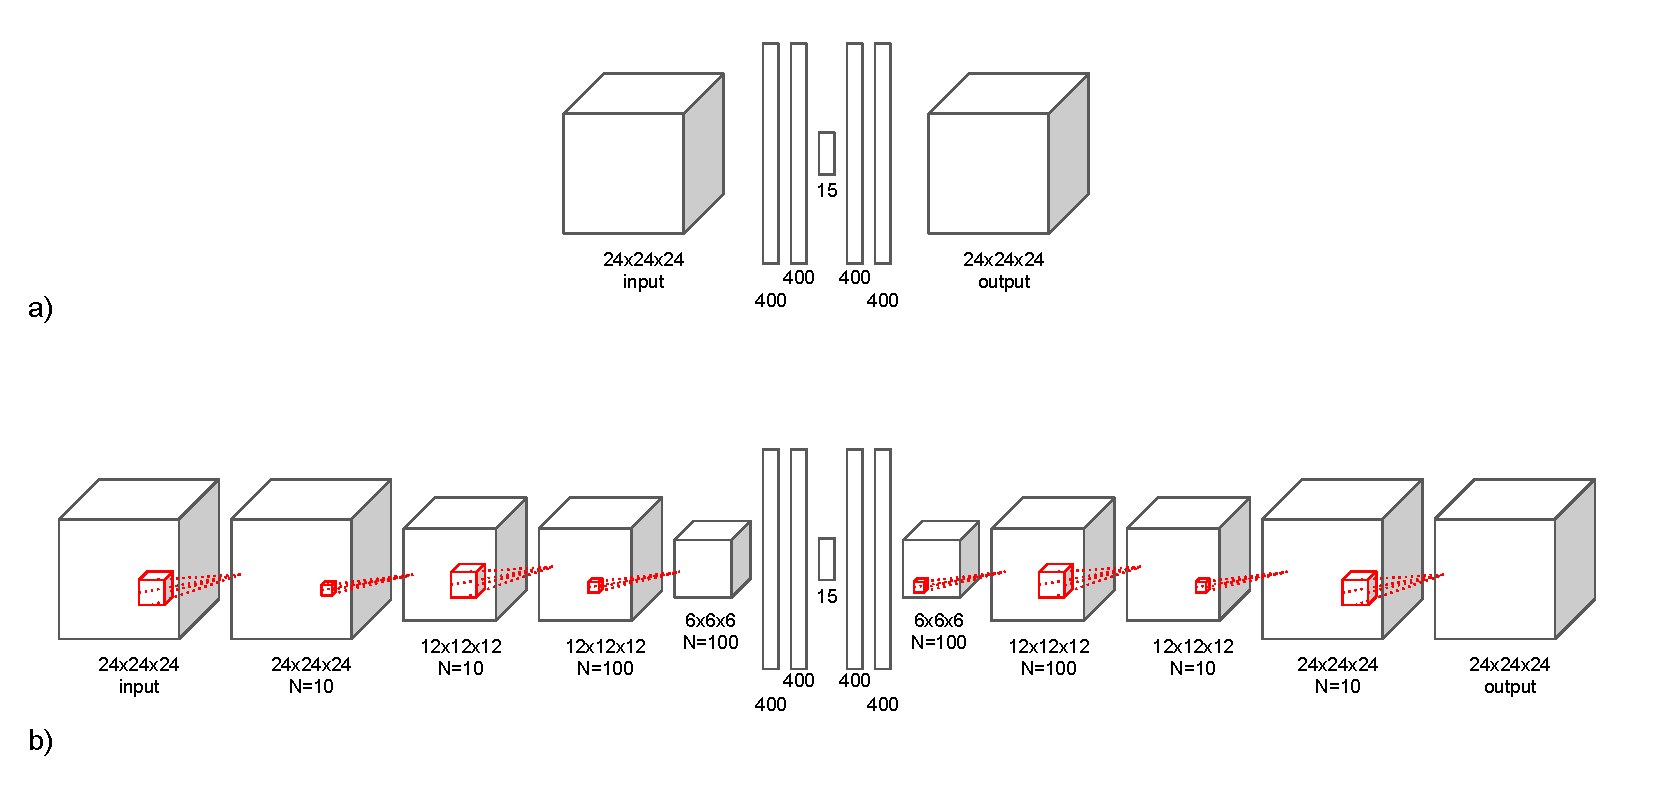
\includegraphics[width=5.2in]{images/architecture.pdf}
  \caption{The SegMatchAE autoencoder architectures. a) The fast architecture. b) The accurate architecture}
  \label{fig:architecture}
\end{figure}

In both architectures, the latent space size is set to 15. To these 15 values predicted by the autoencoder for segment representations, are concatenated 3 dimensional scales, for $x$, $y$, and $z$, which are calculated during voxelization. These are added because the voxelization step scales all segments to fit inside the occupancy grid. Thus, the autoencoder is given dimensionless input in $x$, $y$, and $z$ directions. As such, unless the autoencoder guesses the common size of segments based on other indicators (there is reason to believe that it does not: such information would not improve its reconstruction accuracy, nor do we give it any data during training that would allow such properties to be learnt), size information of the segment would be lost. This gives the SegMatch autoencoder descriptor a total of 18 features.\\

\section{Performance}
\label{sec:ae-performance}

On a desktop computer with no GPU, we measure that the fast model takes on average $<$100 ms to encode 100 segments. The accurate model takes on average 20 seconds. Voxelizing 100 segments takes around 20 ms.\\

With GPU enabled, a 20x speedup is measured on average for the accurate model during training. For encoding, a more modest speedup of around 5x is observed.

\section{Results}
\label{sec:ae-results}

\subsection{Segment Reconstructions}

Our measurements show greater accuracy for the accurate model architecture, as expected (See Fig.~\ref{fig:trainingcost}).\\

\begin{figure}
  \centering
  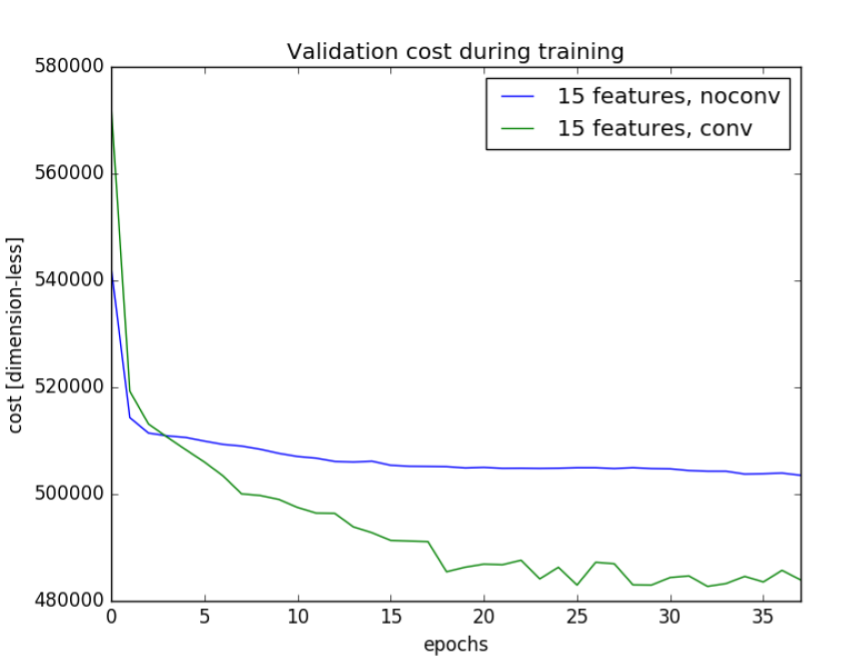
\includegraphics[width=3.2in]{images/trainingcost.png}
  \caption{Comparison of valdidation cost for the fast and accurate architectures, when the same training regime is applied to both, shows that the accurate architecture generalizes better and with greater reconstruction accuracy.}
  \label{fig:trainingcost}
\end{figure}

\begin{figure}
  \centering
  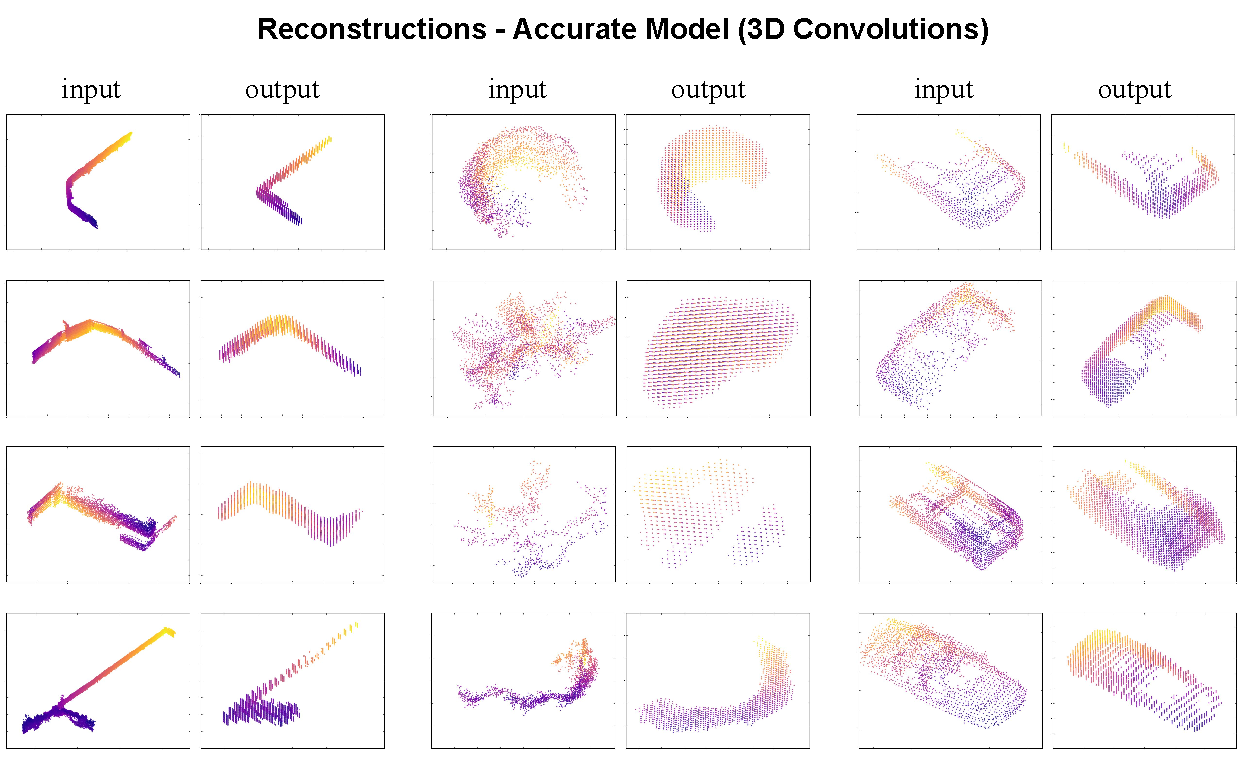
\includegraphics[width=5.2in]{images/convreconstructions.pdf}
  \caption{Comparison of valdidation cost for the fast and accurate architectures, when the same training regime is applied to both, shows that the accurate architecture generalizes better and with greater reconstruction accuracy.}
  \label{fig:trainingcost}
\end{figure}

\begin{figure}
  \centering
  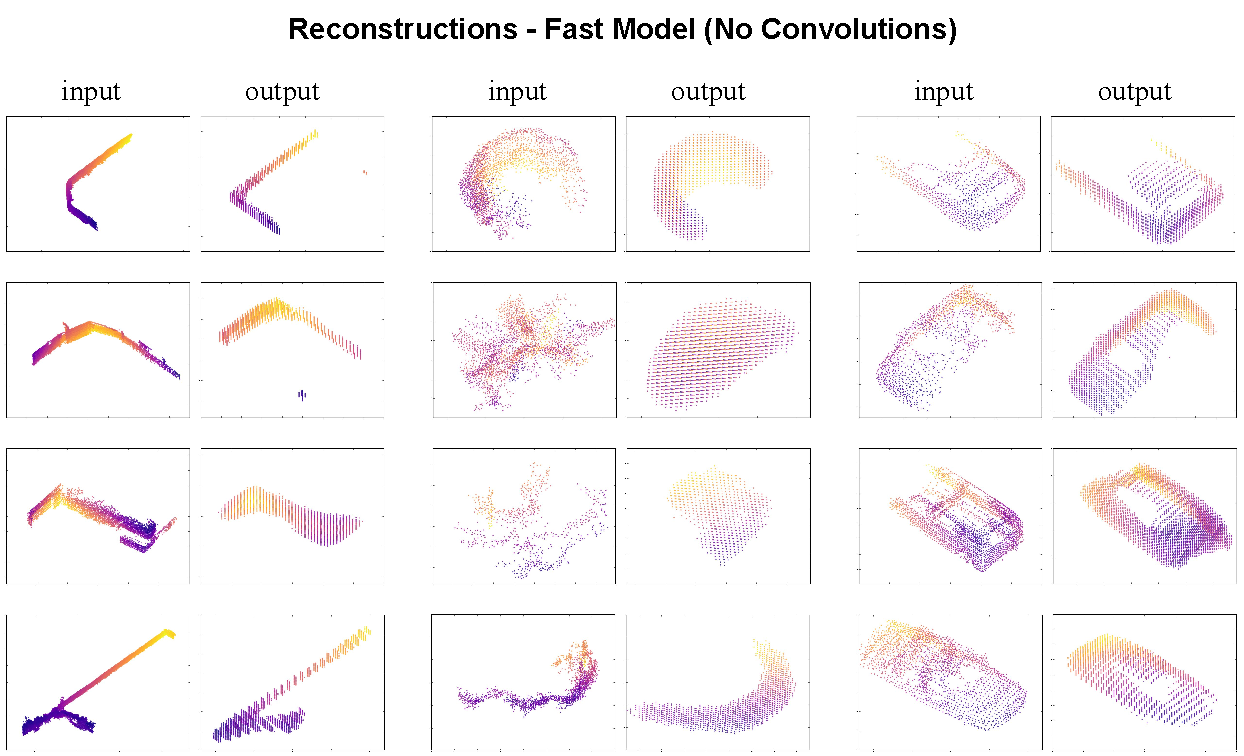
\includegraphics[width=5.2in]{images/noconvreconstructions.pdf}
  \caption{Comparison of valdidation cost for the fast and accurate architectures, when the same training regime is applied to both, shows that the accurate architecture generalizes better and with greater reconstruction accuracy.}
  \label{fig:trainingcost}
\end{figure}

A preprint paper by Brock et al.  \cite{voxel-autoencoder}, published while this project was underway,  mentions successful results on datasets using Variational Autoencoders for reconstructing Voxelized 3D data.
Brock et al. \cite{voxel-autoencoder} report that ``The model attains a 99.39\% true positive and 92.36\% true negative reconstruction accuracy on the ModelNet10 test set, indicating that it learns to reconstruct with high fidelity, but tends to slightly overestimate the probability of a voxel being present. ''\\

In our own experiments, we run the autoencoder on an arbitrary voxelized segment, producing a voxelized reconstruction. The reconstruction is then passed as input to the autoencoder, outputting a reconstruction-reconstruction, and so on 60 times. The goal was to see if the reconstructions tended to converge to a particular shape. We observed that with every iteration, the output prediction contains on average more occupied voxels, resulting in a final reconstruction which is a completely filled voxel. This agrees with the statement from Brock et al. \cite{voxel-autoencoder} quoted in the previous paragraph, which observes that the model ``tends to slightly overestimate the probability of a voxel being present.''\\

Experiments on the ModelNet database \cite{modelnet}, also show reconstruction results in accordance with Brock et al.'s observations.


\subsection{Latent Space}

An intuition is that the accurate architecture, due to having 3D convolutions, would be able to more efficiently compress segment representations in the latent space. Our observations show that on average the accurate model keeps 3 latent dimensions unused, whereas the fast model keeps 1 dimension unused (see Fig.~\ref{fig:fastvaccurate-features}). This goes in accordance with our expectations.\\

\begin{figure}
  \centering
  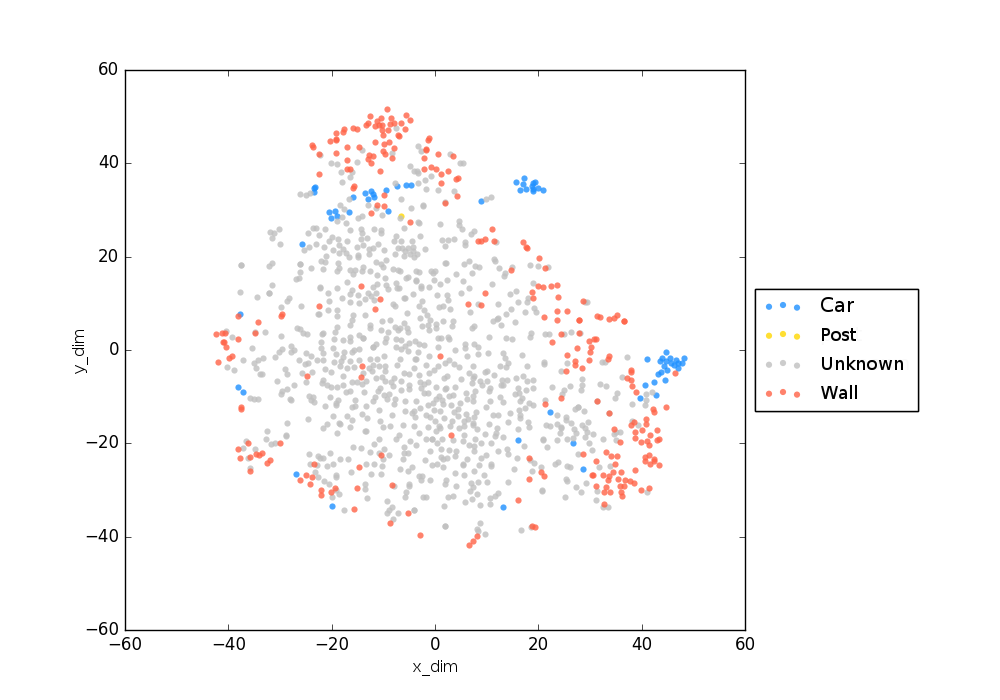
\includegraphics[width=5.2in]{images/t-sne.png}
  \caption{T-SNE projection of the latent space representations for 1000 segments in the KITTI drive 18 dataset.}
  \label{fig:fastvaccurate-features}
\end{figure}

\begin{figure}
  \centering
  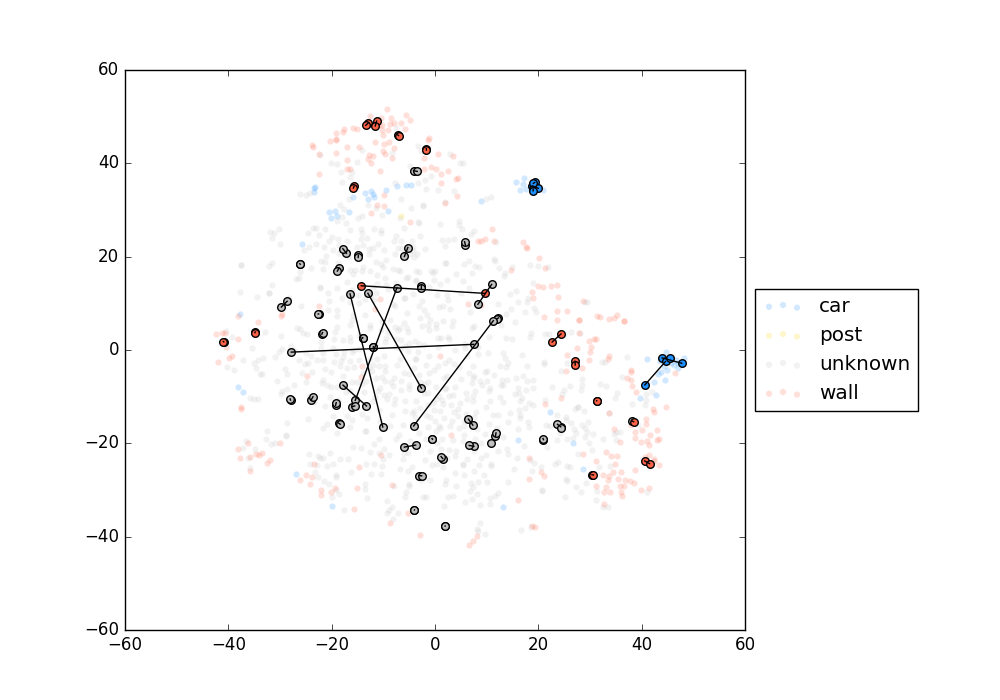
\includegraphics[width=5.2in]{images/t-sne_matches.png}
  \caption{Segment ground truth matches collected during the KITTI drive 18 run, overlaid on their T-SNE projection.}
  \label{fig:fastvaccurate-features}
\end{figure}

\begin{figure}
  \centering
  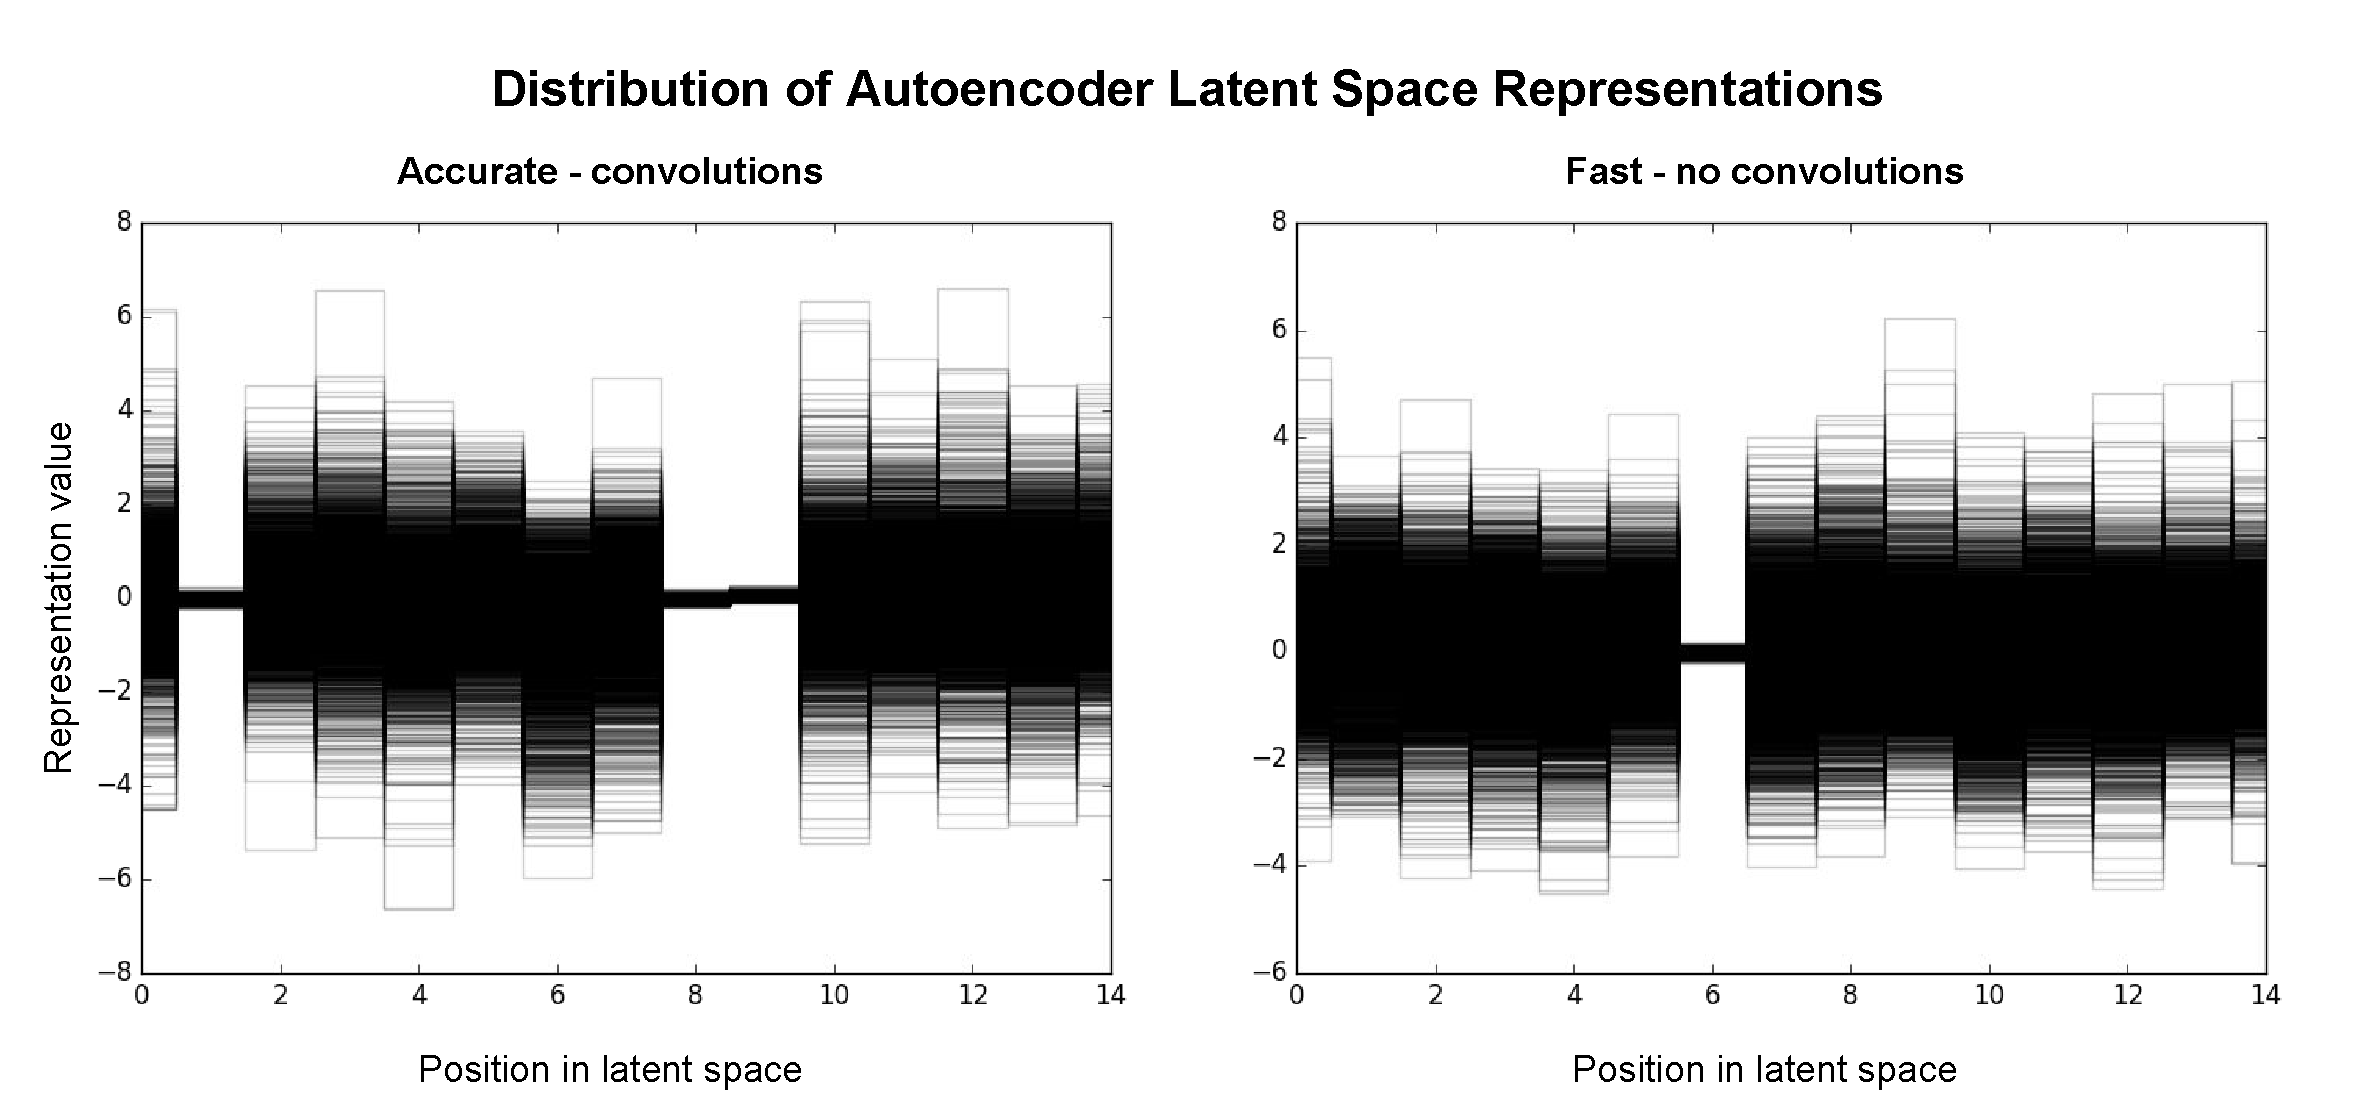
\includegraphics[width=5.2in]{images/fastvaccuratefeatures.pdf}
  \caption{Comparison of the latent space representations for over 1000 segments from the KITTI drive 18 dataset.}
  \label{fig:fastvaccurate-features}
\end{figure}

\subsection{In-the-loop Results}

\begin{figure}
  \centering
  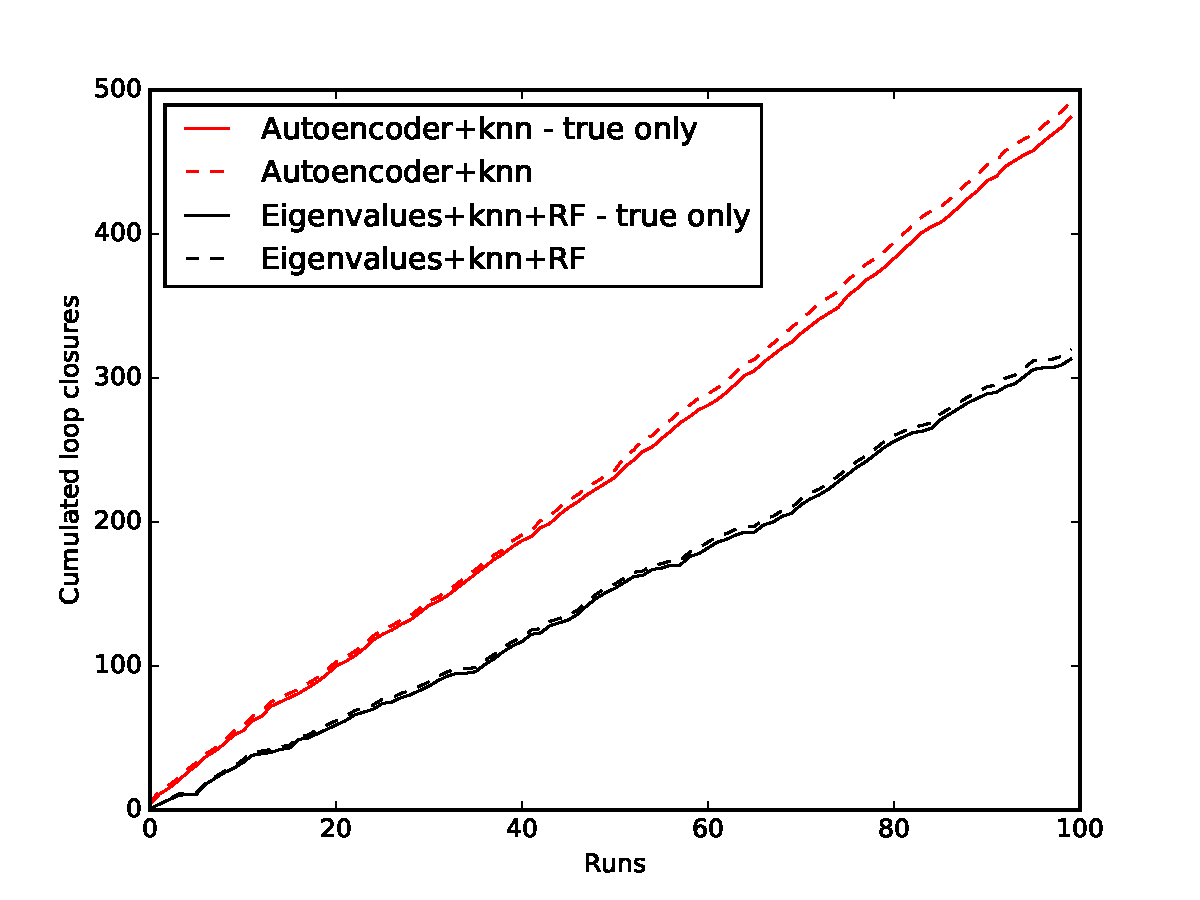
\includegraphics[width=5.2in]{images/kitti20performance.pdf}
  \caption{Accumulated loop closures during 100 runs of SegMatch on the same dataset (KITTI drive 20)}
  \label{fig:kitti20-performance}
\end{figure}

False to True LC ratio - autoencoder: 0.022869022869\\
False to True LC ratio - eigenvalues: 0.0223642172524\\

